\documentclass{article}
\usepackage[letterpaper,landscape,top=2.5cm,bottom=2.5cm,right=2.5cm,left=2.5cm]{geometry}
\usepackage{tikz}
\usepackage{fancyhdr}
\usepackage{lastpage}
\usetikzlibrary{shapes.gates.logic.US,trees,positioning,arrows}

\begin{document}
%------------------------------------------------------------------------------------------
	\pagestyle{fancy}
	\fancyhf{}
	\setlength{\headheight}{15pt}
	\setlength{\headsep}{10pt}
	\lhead{EBSD Plugin Project --- Flow Chart}
	\rhead{\today}
	\lfoot{}
	\rfoot{\thepage/\pageref{LastPage}}
%------------------------------------------------------------------------------------------

\section*{Maps}
\begin{center}
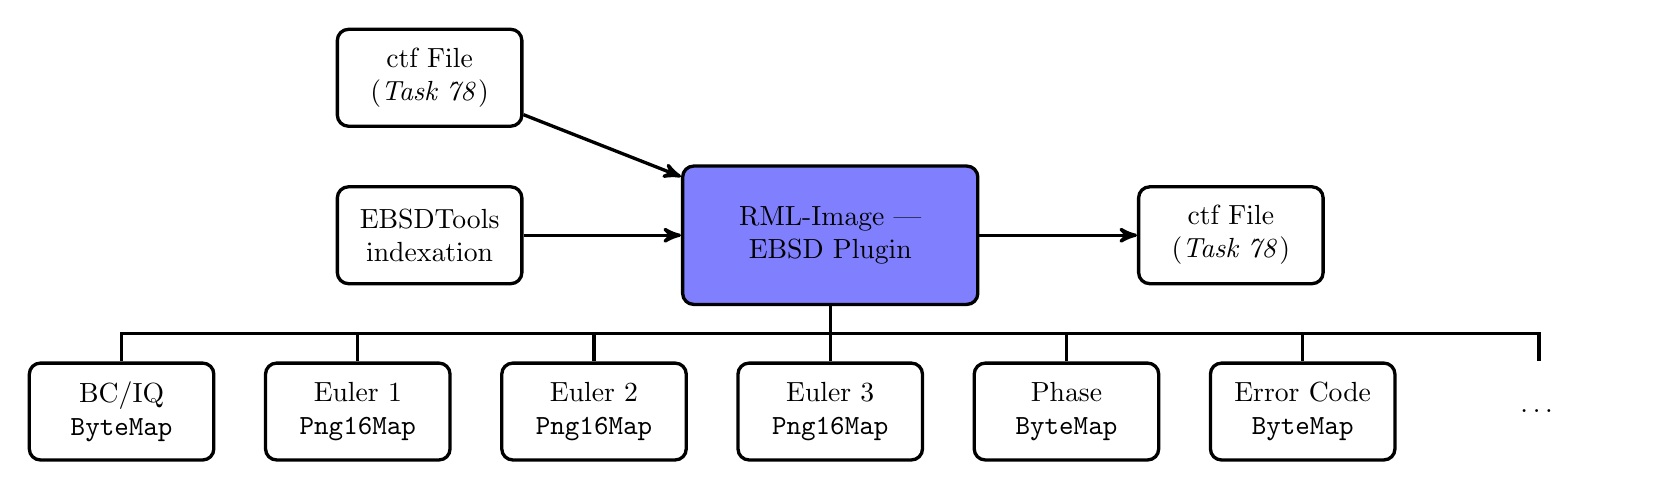
\begin{tikzpicture}[
% Event style
		root/.style={rectangle
							    , rounded corners
							    , fill=blue!50!white
							    , draw=black, very thick
							    , text width=10em
							    , minimum height=5em
							    , text centered
							    , anchor=north},
		event/.style={rectangle
							    , rounded corners
							    , fill=white
							    , draw=black, very thick
							    , text width=6em
							    , minimum height=3.5em
							    , text centered
							    , anchor=north},
		event2/.style={rectangle
%							    , rounded corners
%							    , fill=white
%							    , draw=black, very thick
							    , text width=6em
							    , minimum height=3.5em
							    , text centered
							    , anchor=north},
% Children and edges style
%    edge from parent/.style={very thick,draw=black!70},
		edge from parent path={(\tikzparentnode.south) -- ++(0,-1em)	-| (\tikzchildnode.north)},
    level 1/.style={sibling distance=3cm
                    , level distance=2em
                    , growth parent anchor=south},
    level 2/.style={sibling distance=7cm},
%    level 3/.style={sibling distance=5cm}
%%  For compatability with PGF CVS add the absolute option:
%   absolute
    arbre/.style = {very thick
%			       			, node distance=1.6cm
%			       			, on grid
			       			, >=stealth'}
	]
%% Draw events and edges
		\begin{scope}[arbre]
	    \node [root] (g1)  {RML-Image --- EBSD Plugin}
	      child {node (c1) [event] {BC/IQ \\\texttt{ByteMap}}}
	      child {node (c2) [event] {Euler 1 \\\texttt{Png16Map}}}
	      child {node (c3) [event] {Euler 2 \\\texttt{Png16Map}}}
	      child {node (c4) [event] {Euler 3 \\\texttt{Png16Map}}}
	      child {node (c5) [event] {Phase \\\texttt{ByteMap}}}
	      child {node (c6) [event] {Error Code \\\texttt{ByteMap}}}
	      child {node (c7) [event2] {\ldots}}
	      ;
			\node [event] (g2) [left=of g1, shift={(-1cm,2cm)}] {ctf File \\ (\emph{Task 78})} edge [->] (g1);
			\node [event] (g3) [left=of g1, shift={(-1cm,0)}] {EBSDTools indexation} edge [->] (g1);
			\node [event] (g4) [right=of g1, shift={(1cm,0)}] {ctf File \\ (\emph{Task 78})} edge [<-] (g1);
		\end{scope}
\end{tikzpicture}
\end{center}
%------------------------------------------------------------------------------------------
\newpage
\section*{Post-treatment}
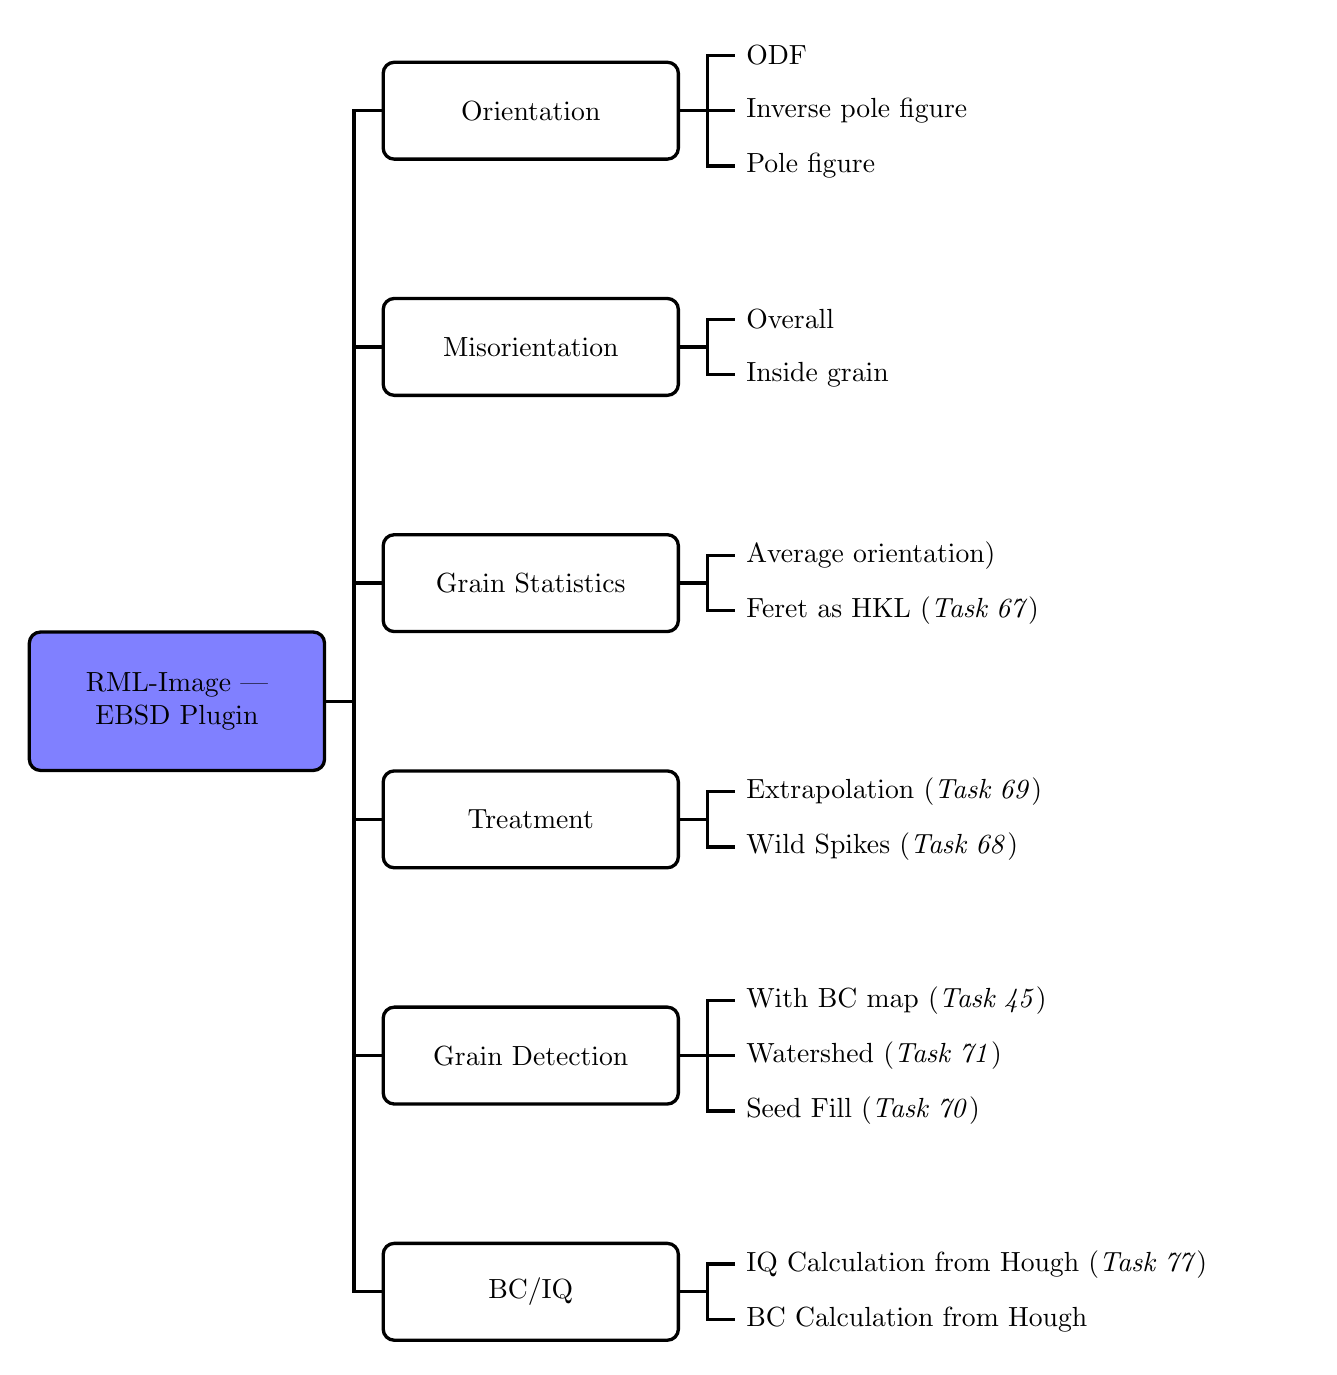
\begin{tikzpicture}[
% Event style
		root/.style={rectangle
							    , rounded corners
							    , fill=blue!50!white
							    , draw=black, very thick
							    , text width=10em
							    , minimum height=5em
							    , text centered
							    , anchor=west},
		event/.style={rectangle
							    , rounded corners
							    , fill=white
							    , draw=black, very thick
							    , text width=10em
							    , minimum height=3.5em
							    , text centered
							    , anchor=west},
		task/.style={rectangle
%							    , rounded corners
							    , fill=white
%							    , draw=black, very thick
							    , text width=20em
							    , minimum height=2em
%							    , text right
							    , anchor=west},
% Children and edges style
%    edge from parent/.style={very thick,draw=black!70},
		edge from parent path={(\tikzparentnode.east) -- ++(1em,0) |- (\tikzchildnode.west)},
%		edge from parent path={(\tikzparentnode.south) -- ++(0,-1em)	-| (\tikzchildnode.north)},
    level 1/.style={sibling distance=3cm
                    , level distance=2em
                    , growth parent anchor=east},
    level 2/.style={sibling distance=2em},
%    level 3/.style={sibling distance=5cm},
%%  For compatability with PGF CVS add the absolute option:
%   absolute
    arbre/.style = {very thick
%			       			, node distance=1.6cm
%			       			, on grid
			       			, >=stealth'}
	]
%% Draw events and edges
		\begin{scope}[arbre]
	    \node [root] (g1)  {RML-Image --- EBSD Plugin} [grow=east]
	      child {node (c1) [event] {BC/IQ}
	        child {node (c1c1) [task] {BC Calculation from Hough}}
	        child {node (c1c2) [task] {IQ Calculation from Hough (\emph{Task 77})}}
	        }
	      child {node (c2) [event] {Grain Detection}
	        child {node (c2c1) [task] {Seed Fill (\emph{Task 70})}}
	        child {node (c2c2) [task] {Watershed (\emph{Task 71})}}
	        child {node (c2c3) [task] {With BC map (\emph{Task 45})}}
	        }
	      child {node (c3) [event] {Treatment}
	        child {node (c3c1) [task] {Wild Spikes (\emph{Task 68})}}
	        child {node (c3c2) [task] {Extrapolation (\emph{Task 69})}}
	        }
	      child {node (c4) [event] {Grain Statistics}
	        child {node (c4c1) [task] {Feret as HKL (\emph{Task 67})}}
	        child {node (c4c2) [task] {Average orientation)}}
	        }
	      child {node (c5) [event] {Misorientation}
	        child {node (c5c1) [task] {Inside grain}}
	        child {node (c5c2) [task] {Overall}}
	        }
	      child {node (c6) [event] {Orientation}
	        child {node (c6c1) [task] {Pole figure}}
	        child {node (c6c2) [task] {Inverse pole figure}}
	        child {node (c6c2) [task] {ODF}}
	        }
      ;
	\end{scope}
\end{tikzpicture}
%------------------------------------------------------------------------------------------
\newpage
\section*{Indexation}
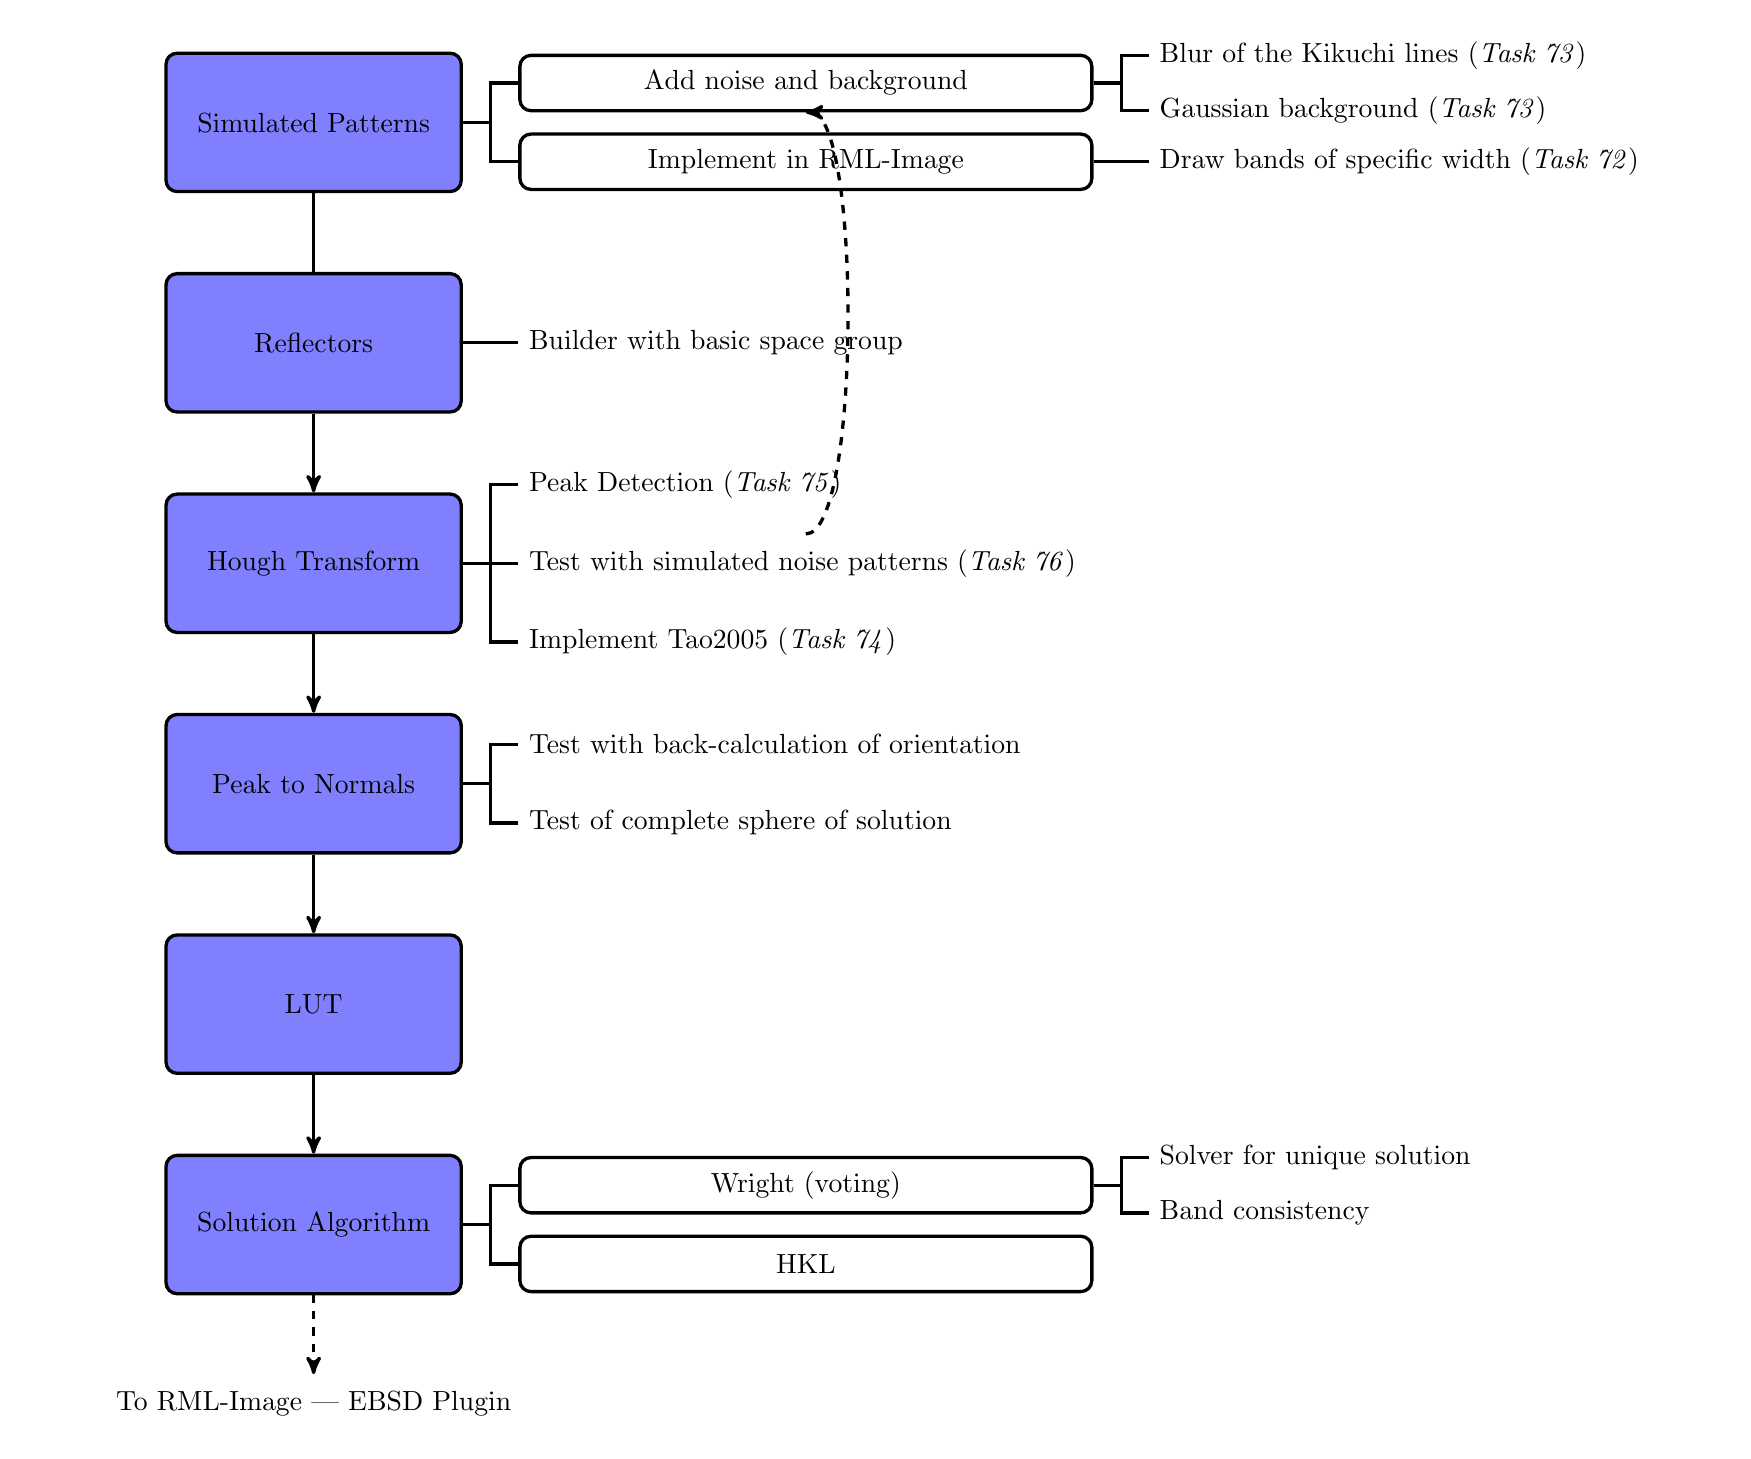
\begin{tikzpicture}[
% Event style
		root/.style={rectangle
							    , rounded corners
							    , fill=blue!50!white
							    , draw=black, very thick
							    , text width=10em
							    , minimum height=5em
							    , text centered
							    , anchor=west},
		event/.style={rectangle
							    , rounded corners
							    , fill=white
							    , draw=black, very thick
							    , text width=20em
							    , minimum height=2em
							    , text centered
							    , anchor=west},
		task/.style={rectangle
%							    , rounded corners
							    , fill=white
%							    , draw=black, very thick
							    , text width=20em
							    , minimum height=2em
%							    , text right
							    , anchor=west},
% Children and edges style
%    edge from parent/.style={very thick,draw=black!70},
		edge from parent path={(\tikzparentnode.east) -- ++(1em,0) |- (\tikzchildnode.west)},
    level 1/.style={sibling distance=1cm
                    , level distance=2em
                    , growth parent anchor=east},
    level 2/.style={sibling distance=2em},
%    level 3/.style={sibling distance=5cm},
%%  For compatability with PGF CVS add the absolute option:
%   absolute
    arbre/.style = {very thick
%			       			, node distance=1.6cm
%			       			, on grid
			       			, >=stealth'}
	]
%% Draw events and edges
		\begin{scope}[arbre]
			\node [root] (g1)  {Simulated Patterns} [grow=east]
	      child {node (g1c1) [event] {Implement in RML-Image}
	        child {node (g1c1c1) [task] {Draw bands of specific width (\emph{Task 72})}}
	      }
	      child {node (g1c2) [event] {Add noise and background}
	        child {node (g1c2c1) [task] {Gaussian background (\emph{Task 73})}}
	        child {node (g1c2c1) [task] {Blur of the Kikuchi lines (\emph{Task 73})}}
	      }
	    ;
	    \node [root] (g1a) [below=of g1] {Reflectors} [grow=east]
	      child {node (g1ac1) [task] {Builder with basic space group}}
      edge (g1);
       
	    \node [root] (g2) [below=of g1a] {Hough Transform} [grow=east]
	      child {node (g2c1) [task] {Implement Tao2005 (\emph{Task 74})}}
	      child {node (g2c2) [task] {Test with simulated noise patterns (\emph{Task 76})}}
	      child {node (g2c3) [task] {Peak Detection (\emph{Task 75})}}
      edge [<-] (g1a);
      
      \node [root] (g3) [below=of g2] {Peak to Normals} [grow=east]
	      child {node (g3c1) [task] {Test of complete sphere of solution}}
	      child {node (g3c2) [task] {Test with back-calculation of orientation}}
      edge [<-] (g2);
      
      \node [root] (g4) [below=of g3] {LUT} [grow=east]
      edge [<-] (g3);
      
      \node [root] (g5) [below=of g4] {Solution Algorithm} [grow=east]
	      child {node (g5c1) [event] {HKL}}
	      child {node (g5c2) [event] {Wright (voting)}
	        child {node (g5c2c1) [task] {Band	consistency}}
	        child {node (g5c2c2) [task] {Solver for unique solution}}
	      }
      edge [<-] (g4);
      
      \node [task, text centered] (g6) [below=of g5] {To RML-Image --- EBSD Plugin} [grow=east]
      edge [dashed, <-] (g5);
      
      \draw[dashed,->] (g2c2.north) .. controls +(2em,0) and +(2em,0) .. (g1c2.south);
	\end{scope}
\end{tikzpicture}

\end{document}
